\documentclass{acm_proc_article-sp}
\usepackage{algorithmic}
\usepackage{algorithm}
\usepackage{listings}
\usepackage{booktabs}
\begin{document}

\title{Re-Allocation of Resources during Releases \titlenote{Copyright information will go here.}}
\numberofauthors{2}
\author{
% 1st. author
\alignauthor
Md Tajmilur Rahman\\
       \affaddr{Concordia University}\\
       \affaddr{Montreal, QC H3G 1M8}\\
       \affaddr{438-932-2288, +1}\\
       \email{rupak.karmadhar@gmail.com}
% 2nd. author
\alignauthor
Peter C. Rigby\\
       \affaddr{Concordia University}\\
       \affaddr{Montreal, QC H3G 1M8}\\
       \affaddr{514-848-2424, +1}\\
       \email{peter.rigby@concordia.ca}
}
\date{20 Oct 2013}
\maketitle
\begin{abstract}
This section will be written at the end.
\end{abstract}
\category{K.6.3}{Software Management}{Software Development; Software Resource Management, Resource Reallocation}
\terms{Experiment, Human Factors, Resource Management, Reallocation}
\keywords{Resource Reallocation, Software Releases} % NOT required for Proceedings
\section{Introduction}
Software projects are notorious for going over budget and schedule. Rush periods are often get seen before a major release that turn the developers into dinosaurs as Frederick Brooks likens in his benchmark study "The Mythical Man Month" \cite{1_brooks}. This "Rush To Release (RTR)" can be prompted either by external forces such as decisions by management to include new features in the release or to release earlier to beat a competitor. Alternatively, the rush may simply be due to inappropriate or unrealistic scheduling. Whatever the reason is it is an obvious. Regardless of the causes, the rush to release stresses developers and often requires developers to work on unusual, high priority or critical areas of the system. In this paper we study how RTR effects project organization and introduces technical debt. The key research questions that we expect to answer with our methodology are as follows:
\begin{enumerate}
\item Do developers work on different areas of the system around the time of release?
\item Are there certain areas of the system that receive increased attention (i.e.\ do developers focus on a smaller set of files around releases)?
\item Do the areas of code that are modified around the time of release have higher defect densities than code that is modified during normal development?
\end{enumerate}

We observe a reallocation of the resources among the software development teams in a large project to identify that an improper reallocation or inappropriate reorganization causes a disruptive event take place in a software development process. We attempt to identify a project’s different release times and calculate the difference between two consecutive releases to discover which are the new areas have been worked between two consecutive releases. The commit log data that we are working on for this purpose will help us to extract a lot of information like calculating the developers' working areas and time-frame of each release. This information will help us to identify the criteria of the resources, their roles, file ownership and nativeness (∆ƞ) in the domain. This knowledge of nativeness (∆ƞ) will guide us understanding the method of reallocation.
Very few research works have been performed regarding the re-allocation of resources.  Robert van Engelen worked for similar kind of a research to understand the resource allocation dynamics across the software projects \cite{2_datta}. He mainly tried to reallocate development resources amongst projects for increasing the satisfactory level of consumer or customer while we are focusing on the impact on code-base like the complexity of script files. Robert proposed a project-entropy metric in his work to understand if there is any limit for a particular reallocation does not lead to user satisfaction. Here entropy is to represent disorder and chaos to understand degradation of software and its inherent complexity. In his work resources may not just be the developers but also can be any other resources necessary for a software project development.
We have organized this paper as follows. In Section 2, we describe some background and motivations followed by some summaries of related works in section 3. Section 4 will describe about the ownership of files and ownership of a set of files or a directories. We will try to understand how native a code-base is to a developer or a development team. In Section 5, some analysis to determine reallocation has been performed in a release or where reallocation needs to be performed will be presented. What changes in nativeness (∆ƞ) occurs after the reallocation. Section 6 will give us the result to show how change in ∆ƞ puts impact on the outcome of a software. Finally section 7 will give us an idea of our future work followed by the conclusion in section 8.

\section{Background}
Sometimes project members with interdependent tasks usually may not communicate effectively; coordination breakdowns occur, which results in integration failures \cite{3_kwan}. There may have lower developers productivity \cite{4_cataldo, 5_damian} which may cause inefficient run in the rush moments in a release period. There is a substantial and important body of literature on risk in software engineering. Boehm identified the most important risks encountered by software project managers and described successful risk management practices \cite{6_boehm, 7_keil, 8_boehm}. Some of the risks identified are related to disruptive events, such as the introduction of a new technology, but most are macro risks associated with running a project, such as developing the wrong functionality. General risk mitigation strategies can be difficult to apply to specific disruptive events. There may be various kinds of disruptive events for example, as a release approaches; developers take shortcuts that introduce technical debt. If it is not repaired, the long term quality of the system will suffer. Another example can be placed, if a lead developer who owns an important part of the code-base leaves and if steps to train other developers were not taken, it will become a dead area of the system and will be difficult to modify and maintain. Also often management reorganizes the developers on a company’s projects, with the result that developers move to code-bases for which they have less experience. The reorganization introduces new perspectives and expertise that can lead to innovation; however, it can also result in a drop in productivity and the unnecessary re-writing of large portions of the system that the new developers do not understand.
In this paper, we plan to take the measures on this last example among them mentioned above. We want to study that proper re-organization or efficient re-allocation of resources based on meaningful criteria can bring better outcome of a software development project by identifying quantify outcomes (Example: number of defects found).

\section{Related Works}
Many people have worked with pretty relevant ideas but I didn't find many very similar to our motivation. Hindle worked on release pattern discovery via partitioning \cite{9_hindle}. In this research they proposed a method of observing, analyzing and summarizing the results of metrics of revisions found near releases. They have characterized a project's behavior around the time of major and minor releases. This is done by partitioning the observed activities like the art-effect check-ins around the dates of major and minor releases, then look for reasonable patterns. Hindle divided the revisions in each release in 4 different classes, Source Code, Testing, Building, and Documentations. Actually this paper worked in a reverse way than Cook did \cite{10_cook}. Cook inserted sensors and monitors into the development process but Hindle and Michael analyzed the data to understand what happened in the past.
Another research work we would like to mention was done by  Damian where they have worked on the role of domain knowledge and cross functional communication among the OOS development teams \cite{11_damian}. Posnett did some dual ecological measures of focus in software development \cite{12_posnett}. Posnett's measure was for the more general view that unifies developer focus and artifact ownership. Posnett analyzed i) developer artifact contribution to network to a predator-prey food web ii) drew upon ideas from ehology to produce a novel and iii) conceptually unified view of measuring focus and ownership. Another study was done by F. Rahman about the authorship of the code-bases in OSS development \cite{13_rahman}.

\section{Methodology and Data}
This section presents our methodology for discovering information which can give us the idea to get the answers to our research questions. We have collected the development history data of Linux kernel. Actually it is a database containing the all the commit log records by the Linux kernel developers since 2005. We are going to present the steps involved in this process and then we will follow up with an application of our methodology in a case study.
Our methodology can be summarized as: Extracting Data for revisions and releases (Section 4.1); Partitioning the version numbers (Section 4.2); Get time-span between each release (Section 4.3); Calculate developer areas (Section 4.4); Finding code area owners (Section 4.5). Finding merging time and development time within a release period that we found in section 4.1 (Section 4.6). 

\subsection{Extracting Data}
We went for the VCS of a target project and either mirror the repository or download each revision and commit log history data individually. From VCSs such as CVS we extract the revisions and release information. We then put them into a database. We have used here PSQL database to create tables in, to store our extracted data. These extracted will be analyzed by us later on. Per each revision the information extracted includes the commit id, tree id, author of the revision, date of revision, the name of the revised file, parent and child info for the revision and the detail log information. Once extraction is complete we are ready to partition the version numbers (Section 4.2) and duration  of each release (Section 4.3).

\subsection{Partioning Release Numbers}
We stored the git commit log extracted data into a table named git commit and git revision where all the basic and log information for a particular commit was mentioned in the first table and second one containing which commit belongs to which version of Linux kernel development and change details like path modified, new path created due to the change, how many addition and how many deletion occurred in a particular commit etc. By joining these tables we can easily get the dates of each version and from the version number which is a combination of different types of releases we can get determine which commit belongs to which version and release, and also what type of release that is as well. Figure 1 shows the picture of the data how it looks like.
\begin{figure}
\centering
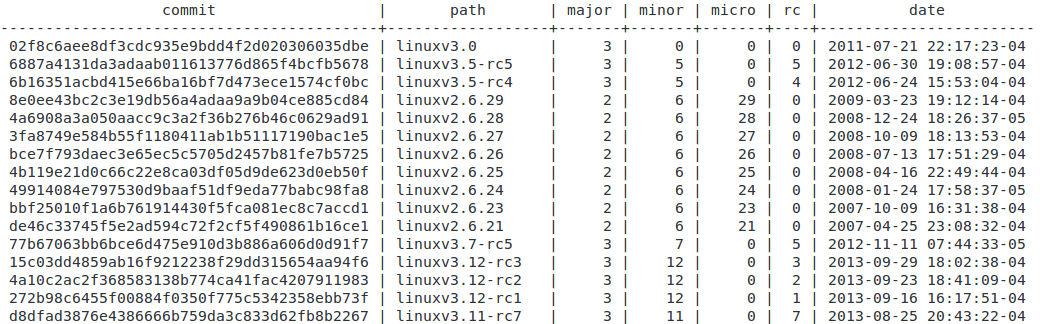
\psfig{file=versions.png, height=1in, width=3in,}
\caption{Releases extracted from Version}
\end{figure}

\begin{lstlisting}
Find out the release candidates:
update git_refs_tags set rc = cast(
  substring(
    path from
      position( '-rc' in path )
        + 3 for 2 
  ) as integer
) where path ~ E'-rc';
\end{lstlisting}
Find out major release version number:
\begin{lstlisting}
update git_refs_tags set major = cast(
  substring(
    path, 'v([0-9]+)\.?'
      ) as integer
);
\end{lstlisting}
Find out minor release version number:
\begin{lstlisting}
update git_refs_tags set minor = cast(
  substring(
    path, 'v[0-9]+\.([0-9]+)\.?'
      ) as integer
);
\end{lstlisting}
Find out micro release version number:
\begin{lstlisting}
update git_refs_tags set micro = cast(
  substring(
    path, 'v[0-9]+\.[0-9]+\.([0-9]+)\-?'
      ) as integer
);
\end{lstlisting}

We are getting the release dates also with every commit record. So we can understand which commit belongs to which version of release, is this a major release or minor or micro. Another information we have captured that is \textbf{rc} which means that the particular commit was for a release candidate.

\subsubsection{Explanation}
A Linux kernel development release version having maximum length of information looks like \textbf{linuxvA.B.C-rcP} where A, B, C, P are numeric. If a release versioning looks like ``linuxv2.6.13'' it tells us that this particular release is the 13th minor release  under  the 6th major release of kernel version 2. ``linuxv2.6.13\textbf{-rc1}'' says that after the 13th minor release been released development for the next release has been started and rc1 is the first candidate on the way to the next release. It doesn't ensure that next release is also going to be another minor release.

\subsection{Get Time-Span Between Release}
Another information that we require is what are the durations of the releases of Linux kernel development. To achieve that we joined the table shown in figure 1 and git\_commit. The following psql query did the job pretty easily for us:
\begin{lstlisting}
select
grt.path as release, grt.major, grt.minor,
grt.micro, grt.rc, gc.committer_dt
from
git_refs_tags grt, git_commit gc
where
gc.commit = grt.commit
order by
gc.committer_dt
\end{lstlisting}
This query gives us all the dates of commit for each and every release, so we can easily find out the duration between two consecutive releases. This information is more important to us because we need to see what is the actual development period and what is the merging or other fixing period within a release time-span and also we need to understand how developers are working, what is the impact of their changes made in the code-base during a particular release period. Table 1 shows a small portion of this information. Preior to calculate the areas of the developers in secion 4.4 we require this information.

\begin{table}[ht]
\caption{Nonlinear Model Results}	 % title of Table
\centering 						% used for centering table
\begin{tabular}{c c c c}				% centered columns (4 columns)
\hline\hline						%inserts double horizontal lines
% table heading
Release & Type & Start Date & End Date \\ [0.5ex]
\hline 							% single horizontal line
% inserting body of the table
linuxv2.6.12-rc2 & rc       & 2005-04-16 & 2005-04-16 \\
linuxv2.6.12-rc3 & rc       & 2005-04-16 & 2005-04-20 \\
linuxv2.6.12-rc4 & rc       & 2005-04-20 & 2005-05-07 \\
linuxv2.6.12-rc5 & rc       & 2005-05-07 & 2005-05-24 \\
linuxv2.6.12-rc6 & rc       & 2005-05-24 & 2005-06-06 \\
linuxv2.6.12        & micro & 2005-06-06 & 2005-06-17 \\
linuxv2.6.13-rc1 & rc       & 2005-06-17 & 2005-06-29 \\
linuxv2.6.13-rc2 & rc       & 2005-06-29 & 2005-07-05 \\
linuxv2.6.13-rc3 & rc       & 2005-07-05 & 2005-07-13 \\
linuxv2.6.13-rc4 & rc       & 2005-07-13 & 2005-07-28 \\
linuxv2.6.13-rc5 & rc       & 2005-07-28 & 2005-08-02 \\
linuxv2.6.13-rc6 & rc       & 2005-08-02 & 2005-08-07 \\
linuxv2.6.13-rc7 & rc       & 2005-08-07 & 2005-08-23 \\
linuxv2.6.13        & micro & 2005-08-23 & 2005-08-28 \\
linuxv2.6.14-rc1 & rc       & 2005-08-28 & 2005-09-12 \\
linuxv2.6.14-rc2 & rc       & 2005-09-12 & 2005-09-19 \\
linuxv2.6.14-rc3 & rc       & 2005-09-19 & 2005-09-30 \\
linuxv2.6.14-rc4 & rc       & 2005-09-30 & 2005-10-10 \\
linuxv2.6.14-rc5 & rc       & 2005-10-10 & 2005-10-20 \\
[1ex]							% adds vertical space
\hline 							% inserts single line
\end{tabular}
\label{table:nonlin} 				% is used to refer this table in the text
\end{table}

\subsection{Calculate Developers' Area}
Developers are working throughout the release time. Developers' are means the files developers work in. But it doesn't refer the to file itself but to understand which files are being touched by which developers. We see that authors are committing files almost everyday throughout a release. We have the commit log data in our hand and we know what is the duration of each releases (i.e.\ start and end dates). Now it is possible to find out which commits were made for which files by a developer within a given time range of a release.

We select all the release information from the table where we stored the releases with their corresponding time-span. After that we select author name and other relevant information from the joining of ``git\_revision'' and ``git\_commits'' tables for every release. We insert these information into a table named ``dev\_area\_rel'' so that we can use the data for our further analysis.

The following pseudo code may show the path to achieve the desired result in this section:

\begin{algorithm}
\caption{Calculate Developers Area}
\begin{algorithmic}
\REQUIRE $ $\\
$commit\_date \geq  release\_start\_date$\\
$commit\_date < release\_end\_date$
\ENSURE
\STATE $get all releases$

\WHILE{$prev\_release\_date \leftarrow release\_start\_date and release \leftarrow release\_version$}
\IF{$release$}
	\IF{$commit\_date \geq  release\_start\_date$ and $commit\_date < release\_end\_date$}
		\STATE $select author, path, commits, churn$
		\STATE $insert data into table dev\_area\_rel$
	\ENDIF
\ENDIF
\ENDWHILE
\end{algorithmic}
\end{algorithm}

\subsection{Finding Code-Area Owners}
... ... ...

\subsection{Jaccard Distance}
Once we found different releases and the release periods as well we calculate the developers' are to see what changes developers are doing in releases. We also want to know what is the difference being created by making changes between two consecuitive releases. If I explain it more then I can say, developers are working in many different files in a release and may work in a same file again for the next release or releases. 

\section{Conclusions}
This section will be written at the end.
%\end{document}  % This is where a 'short' article might terminate

\section{Acknowledgments}
... ... ...
\bibliographystyle{abbrv}
\bibliography{paper1} 
\appendix
%Appendix A
\section{Headings in Appendices}
Apendix section will be written later with the following subsections may be:
\subsection{Introduction}
...
\subsection{Background and Motivation}
\subsubsection{Related Works}
...
\subsubsection{Methodology and Data}
...
\subsection{Conclusions}
...
\subsection{Acknowledgments}
...

\subsection{References}
... ...

\balancecolumns
\end{document}